
\chapter{Monitorização de Serviços com OpenTelemetry}

\section{Introdução e Caracterização do Sistema Monitorado}

O cenário atual do desenvolvimento de software é marcado pela crescente adoção de arquiteturas de microsserviços e ambientes \textit{cloud-native}, suportados por plataformas de orquestração como o Kubernetes. Embora esta abordagem promova agilidade, escalabilidade e resiliência, também introduz uma complexidade significativa, especialmente no monitorização e na depuração de sistemas distribuídos. A proliferação de serviços independentes, cada um com a sua própria lógica e ciclo de vida, bem como a comunicação assíncrona entre eles, torna o seguimento de uma única requisição de ponta a ponta uma tarefa desafiadora.

Neste contexto, a monitorização avançada torna-se uma disciplina fundamental para garantir a fiabilidade, o desempenho e a resiliência destes sistemas distribuídos \cite{Salah2017}.


\subsection{Visão geral da Arquitetura do Sistema R2UT}

A arquitetura do R2UT segue os princípios das arquiteturas de microsserviços com o objetivo de garantir flexibilidade, escalabilidade e resiliência na gestão do ciclo de vida da construção modular. Esta arquitetura é composta por diversos componentes (ou módulos), cada um responsável por uma funcionalidade específica. A estrutura modular facilita a manutenção, o desenvolvimento e a integração de novas capacidades sem impactar a operação dos restantes serviços.

A solução está organizada em camadas, sendo que cada serviço é executado de forma isolada num \textit{container} Docker, posteriormente gerido e orquestrado pelo Kubernetes. Esta abordagem permite que os serviços operem de forma autónoma, escalando conforme necessário de acordo com a carga e as necessidades operacionais. A comunicação entre os serviços é assegurada através de \textit{REST APIs}, \textit{gRPC} e mensagens via \textit{Kafka}, permitindo interoperabilidade eficiente tanto em cenários síncronos como assíncronos.

Além disso, a comunicação entre os diferentes componentes é realizada através de interfaces bem definidas, assegurando um elevado nível de desacoplamento entre os microsserviços e promovendo uma arquitetura extensível, robusta e facilmente evolutiva.


\subsection{Papel do Kubernetes na Arquitetura do R2UT}

O Kubernetes desempenha um papel central na arquitetura do R2UT, fornecendo a infraestrutura necessária para orquestrar e gerir os \textit{containers} dos microserviços e garantindo, entre outras coisas:

\begin{itemize}
    \item \textbf{Escalabilidade automática (\textit{auto-scaling}).} O Kubernetes permite que os \textit{pods} (unidades de execução de \textit{containers}) sejam escalados automaticamente com base na carga de trabalho e na demanda de recursos. Isso é essencial para garantir que o sistema possa lidar com picos de utilização sem comprometer o seu desempenho, como no caso de um aumento de utilizadores que acedem simultaneamente aos serviços.

    \item \textbf{Alta disponibilidade (\textit{High Availability} — HA).} O Kubernetes garante que, caso um \textit{pod} falhe, outro seja automaticamente reiniciado num nó diferente do cluster, minimizando o impacto de falhas no sistema. Isso permite assegurar que os serviços essenciais, como autenticação ou autorização de utilizadores e dispositivos, ou mesmo a gestão de dispositivos IoT, continuem operando sem interrupção.

    \item \textbf{Gestão de \textit{containers}.} O Kubernetes permite gerir a execução de \textit{containers}, garantindo que todos os microsserviços estejam devidamente implantados e funcionando corretamente. Além disso, facilita a atualização e a implementação de novas versões dos serviços, assegurando a inexistência de tempos de inatividade por meio de \textit{rolling update}.

    \item \textbf{Orquestração e balanceamento de carga.} O Kubernetes pode ser configurado para balancear automaticamente a carga de trabalho entre diferentes réplicas de um serviço, garantindo que o tráfego seja distribuído de maneira eficiente, sem sobrecarregar nenhum servidor individualmente. Essa orquestração é crucial para garantir que as interações entre os microsserviços sejam rápidas e confiáveis.
\end{itemize}



\subsection{Arquitetura de Microsserviços no Kubernetes}


A plataforma R2UT é composta por diversos serviços que interagem entre si, cada um implementado como um microsserviço em \textit{containers}. Esses serviços são organizados num cluster Kubernetes, no qual a comunicação entre os componentes é feita através de APIs e de mensagens assíncronas via Kafka. Isto permite que o sistema seja altamente escalável e eficiente. De seguida, destacam-se alguns dos componentes chave desta arquitetura:

\begin{itemize}
    \item \textbf{Base de dados global.} Uma base de dados partilhada por todos os serviços que necessita de escalabilidade horizontal. O Kubernetes facilita a gestão de bases de dados distribuídas, como as suportadas por PostgreSQL com Citus, garantindo elevada performance nas consultas e capacidade de escala.

    \item \textbf{Middleware e plataforma em nuvem.} Serviços responsáveis pela interoperabilidade entre os sistemas internos e pela gestão da infraestrutura na nuvem. O Kubernetes gere os recursos necessários para escalar estes serviços conforme as necessidades de tráfego, facilitando a implementação contínua das aplicações.

    \item \textbf{Módulos específicos.} \textit{Tenant Management}, \textit{Ticket Management}, \textit{PDFBuilder}, \textit{IoT Manager}, \textit{Rules Engine}, \textit{DAE Authentication} são módulos da arquitetura. Cada um opera de forma independente em \textit{containers}, com comunicação entre serviços mediada através de APIs e filas de mensagens (Kafka).

    \item \textbf{Cluster Kafka.} O Kafka é utilizado como \textit{broker} de mensagens para garantir a comunicação assíncrona entre os microsserviços, especialmente quando é necessário gerir grandes volumes de dados e eventos gerados por dispositivos IoT ou interações de utilizadores. O Kubernetes permite a escalabilidade do Kafka através de clusters e réplicas dos \textit{brokers}, assegurando alta disponibilidade e tolerância a falhas.
\end{itemize}


\subsection{Desafios da Monitorização em Sistemas Distribuídos}

A implementação de sistemas distribuídos, como o ambiente Kubernetes com microsserviços, cria desafios significativos em relação à monitorização distribuída. A complexidade do sistema aumenta devido à comunicação assíncrona entre os serviços, à escalabilidade dinâmica dos \textit{pods} e à necessidade de correlacionar eventos gerados por diferentes componentes. A deteção de falhas ponta a ponta e a análise de métricas, \textit{logs} e \textit{traces} de forma eficiente são cruciais para garantir a saúde e o desempenho do sistema. 

Uma monitorização eficaz exige que o sistema seja capaz de capturar, correlacionar e analisar as interações entre os microsserviços, além de acompanhar de forma contínua as métricas de desempenho, os \textit{logs} estruturados e os \textit{traces} distribuídos.


\section{Objetivos e Justificativa da Implementação}

\subsection{Objetivos Práticos}

A principal motivação para a implementação desta solução foi a necessidade de garantir uma visibilidade completa sobre o comportamento do sistema, oferecendo informação em tempo real sobre a saúde e o desempenho da aplicação. O objetivo foi criar uma solução de monitorização avançada integrada que permitisse à equipa de desenvolvimento atuar de forma proativa. Os objetivos práticos da implementação incluem:

\begin{enumerate}
    \item \textbf{Visibilidade em tempo real.} Fornecer uma visão consolidada e interativa do comportamento da aplicação, com a capacidade de monitorizar métricas, \textit{logs} e \textit{traces} de forma centralizada. Isto permite a deteção imediata de anomalias, minimizando o impacto no desempenho e na experiência do utilizador.

    \item \textbf{Redução do MTTR (\textit{Mean Time to Resolution}).} Diminuir o tempo necessário para identificar e resolver problemas. A correlação de dados de diferentes fontes (métricas, \textit{logs} e \textit{traces}) é fundamental para diagnosticar falhas de forma eficiente, permitindo identificar rapidamente a sua causa.

    \item \textbf{Otimização de desempenho.} Capacitar a equipa de desenvolvimento a identificar gargalos e áreas de melhoria da solução antes que estes afetem os utilizadores finais. O uso de alertas e \textit{dashboards} permite otimizar o sistema, ajustando componentes e recursos de acordo com a carga e as necessidades operacionais.
\end{enumerate}

Nesta fase, importa referir que o foco da solução de monitorização foi deliberadamente delimitado aos microsserviços desenvolvidos internamente pela equipa do projeto, nomeadamente os módulos responsáveis pela gestão de \textit{tickets}, gestão de utilizadores, dispositivos IoT, autenticação, regras e serviços de apoio à plataforma. Assim, a monitorização abrange apenas os componentes proprietários da plataforma R2UT, excluindo serviços externos ou de terceiros (como bases de dados geridas por fornecedores, APIs externas ou serviços \textit{cloud} nativos). Esta decisão foi motivada pela necessidade de garantir visibilidade e controlo direto sobre os módulos sob responsabilidade da equipa, assegurando que o esforço de instrumentação se concentra nas partes do sistema onde é possível atuar de forma proativa.


\section{O Papel do OpenTelemetry na Monitorização de Microsserviços}

Em arquiteturas de microsserviços, nas quais diversos serviços isolados cooperam para servir uma única requisição, rastrear o comportamento global do sistema torna-se um desafio. Problemas como latência entre serviços, falhas silenciosas ou dependências ocultas exigem que a monitorização vá além das abordagens tradicionais. Nesse contexto, o \textit{OpenTelemetry} surge como uma camada padronizada de telemetria, capaz de unificar métricas, \textit{logs} e \textit{traces} e de oferecer correlação ponta a ponta, com menor acoplamento ao \textit{backend}.

\subsection{O que é o \textit{OpenTelemetry}}

O \textit{OpenTelemetry} (\textit{OTel}) é um projeto \textit{open-source} da \textit{CNCF} que fornece \textit{API}, \textit{SDK} e o \textit{OpenTelemetry Collector} para instrumentar e transportar os três sinais de telemetria - \textit{traces}, métricas e \textit{logs} - de forma agnóstica ao fornecedor e independente do \textit{backend}. O objetivo é padronizar a geração e exportação de telemetria, permitindo encaminhar os dados para sistemas como \textit{Prometheus}, \textit{Jaeger}, \textit{Loki} e outros, sem necessidade de alterações no código da aplicação.

O \textit{Collector} atua como um binário \textit{vendor-agnostic} que recebe, processa e exporta telemetria para um ou múltiplos destinos, removendo a necessidade de operar coletores específicos por ferramenta e suportando protocolos abertos como \textit{OTLP}, \textit{Prometheus} e \textit{Jaeger}, entre outros.


\subsection{Principais Componentes}

Embora os detalhes sejam explicados nas secções seguintes, vale apresentar aqui os blocos conceptuais do \textit{OpenTelemetry}. São eles:

\begin{itemize}
    \item \textbf{APIs / SDKs / Instrumentação.} As \textit{API} definem o contrato genérico para rastreamento, métricas e \textit{logs}, enquanto os \textit{SDKs} concretizam esse contrato em cada linguagem, permitindo tanto a instrumentação manual como automática.
    
    \item \textbf{Exporters / Receivers.} Componentes responsáveis por enviar ou receber telemetria em formatos como \textit{OTLP}, \textit{Jaeger} e \textit{Prometheus}.
    
    \item \textbf{Collector.} Componente neutro que organiza \textit{pipelines} (\textit{receivers -- processors -- exporters}), permitindo filtragem, enriquecimento, amostragem e distribuição (\textit{fan-out}) de telemetria.
\end{itemize}

Todos estes componentes trabalham em conjunto para garantir que a telemetria gerada pelo sistema seja relevante, consistente e útil para análise.

\subsection{Sinais, Convenções Semânticas e Recursos}

O \textit{OpenTelemetry} organiza as ações de monitorização em três sinais principais:

\begin{itemize}
    \item \textbf{Traces}, que descrevem operações distribuídas através de \textit{spans} correlacionados;
    \item \textbf{Métricas}, que representam valores quantitativos observados ao longo do tempo;
    \item \textbf{Logs estruturados}, que contêm registos detalhados de eventos com contexto adicional.
\end{itemize}

Para permitir comparações entre serviços e linguagens, o \textit{OTel} define convenções semânticas (\textit{Semantic Conventions} - \textit{SemConv}), um vocabulário padronizado para atributos relacionados com \textit{HTTP}, bases de dados, envio de mensagens e outros domínios. 

Além disso, atributos de \textit{Resource} (como \texttt{service.name}, \texttt{service.version}, \texttt{service.namespace}) identificam consistentemente a origem da telemetria. A aplicação sistemática das \textit{SemConv} melhora a filtragem, correlação e exploração nos \textit{dashboards} - \texttt{service.name} é um dos atributos obrigatórios.


\subsection{Vantagens, Limitações e Desafios do OpenTelemetry}

A adoção do \textit{OpenTelemetry} traz benefícios substanciais no contexto de arquiteturas distribuídas, sobretudo ao padronizar a recolha de telemetria e ao oferecer uma integração unificada para diversos tipos de sinais e plataformas. No entanto, tal como qualquer tecnologia emergente, implica também alguns desafios que precisam ser considerados.

\textbf{Vantagens}

\begin{itemize}
    \item \textbf{Padronização e portabilidade.} Uma única camada de instrumentação permite recolher telemetria de diferentes serviços e enviá-la para múltiplas ferramentas, reduzindo dependência de fornecedores e minimizando esforços em processos de migração ou integração.
    
    \item \textbf{Flexibilidade através do Collector.} O \textit{OpenTelemetry Collector} oferece grande capacidade de adaptação, suportando exportação para múltiplos destinos, mecanismos de \textit{buffering} e \textit{retry}, amostragem inteligente e enriquecimento de dados antes do armazenamento, tudo num ponto central da arquitetura.
    
    \item \textbf{Aderência ao ecossistema \textit{cloud-native}.} A ferramenta foi concebida para ambientes modernos, com suporte maduro para Kubernetes, serviços distribuídos e \textit{auto-instrumentation} disponível para várias linguagens, incluindo .NET.
\end{itemize}

A adoção do \textit{OpenTelemetry}, contudo, não está isenta de desafios. A complexidade de sistemas distribuídos faz com que a instrumentação, operação e gestão da telemetria requeiram planeamento cuidadoso e boas práticas consolidadas.

\textbf{Limitações e Desafios}

\begin{itemize}
    \item \textbf{Curva de configuração e operação.} Pipelines mal definidas podem provocar perda de dados, latências adicionais ou sobrecarga em recursos. O próprio Collector necessita de configuração cuidada e monitorização contínua.
    
    \item \textbf{Maturidade heterogénea entre sinais.} Embora \textit{tracing} e métricas estejam altamente estabilizados, a componente de logs continua em evolução e pode depender mais de integrações com ferramentas externas, como Loki ou ELK.
    
    \item \textbf{Necessidade de stack complementar.} O \textit{OpenTelemetry} fornece coleta e processamento, mas não inclui armazenamento ou visualização, tornando obrigatória a utilização de ferramentas adicionais como Prometheus, Jaeger, Loki ou Grafana para consulta e análise.
\end{itemize}

\break


\section{Comparação entre OpenTelemetry e a Stack Tradicional de Monitorização (Prometheus, Grafana, Jaeger e Loki)}


Antes de procedermos à comparação das diferentes alternativas, importa clarificar que a análise estabelecida entre \textit{OpenTelemetry} e a \textit{stack} composta por Prometheus, Grafana, Jaeger e Loki não deve ser interpretada como uma avaliação entre ferramentas equivalentes ou mutuamente exclusivas. O \textit{OpenTelemetry} não é um \textit{backend} de armazenamento ou visualização de dados. O seu papel situa-se na camada de instrumentação, recolha, normalização e encaminhamento de telemetria (métricas, rastreamentos e registos).

Ou seja, o \textit{OpenTelemetry} atua como um padrão unificador para a geração e transporte de telemetria, permitindo que diferentes linguagens, bibliotecas e serviços emitam dados num formato consistente (OTLP), que podem ser processados e exportados através do \textit{Collector}. Por contraste, a \textit{stack} tradicional composta por Prometheus, Grafana, Jaeger e Loki cobre essencialmente funções de armazenamento persistente, consulta e visualização dos dados recolhidos.

\begin{itemize}
\item Prometheus realiza a recolha e o armazenamento de séries temporais de métricas, com consultas via PromQL.
\item Grafana fornece visualização e gestão de alertas sobre métricas, logs e outros dados operacionais.
\item Jaeger armazena e permite consultar rastreamentos distribuídos.
\item Loki gere a ingestão e consulta de logs.
\end{itemize}

Assim, mesmo com \textit{OpenTelemetry}, continuam a ser necessários sistemas de \textit{backend} que garantam a persistência e exploração dos dados. A comparação, portanto, reflete abordagens arquiteturais distintas:

\begin{itemize}
\item No modelo tradicional, cada ferramenta exige o seu próprio \textit{agent} ou \textit{exporter}, resultando numa coleta fragmentada.
\item Com \textit{OpenTelemetry}, a instrumentação e coleta são unificadas, e os mesmos dados podem ser enviados para múltiplos \textit{backends}.
\end{itemize}

Deste modo, o \textit{OpenTelemetry} não substitui os \textit{backends} clássicos; complementa-os ao introduzir uma camada padronizada e de abstração que reduz o acoplamento e aumenta a portabilidade da telemetria.

A Tabela \ref{tab:otel_vs_tradicional} resume as principais diferenças entre as duas abordagens, destacando aspetos como instrumentação, padronização e flexibilidade arquitetural.

\begin{table}[h!]
\centering
\caption{Comparação entre OpenTelemetry e a \textit{stack} tradicional de monitorização}
\label{tab:otel_vs_tradicional}
\begin{tabular}{|p{4cm}|p{5cm}|p{5cm}|}
\hline
\textbf{Característica} & \textbf{OpenTelemetry (OTel)} & \textbf{Prometheus + Grafana + Jaeger + Loki} \\ \hline

Instrumentação & Unificada (traces, métricas, logs) & Separada por ferramenta \\ \hline
Padronização & Convenções Semânticas (\textit{SemConv}) & Cada ferramenta define o seu padrão \\ \hline
Agnosticidade de \textit{backend} & Sim, exporta para múltiplos destinos & Não, acoplado a cada \textit{backend} \\ \hline
\textit{Collector} Centralizado & Sim, pipelines flexíveis & Não, coletores independentes \\ \hline
\textit{Auto-instrumentação} & Suporte amplo & Limitado por ferramenta \\ \hline
Dependência de fornecedor & Baixa & Média / Alta \\ \hline
Escalabilidade & Elevada & Elevada, mas com mais componentes dedicados \\ \hline
Curva de aprendizagem & Moderada (pipelines OTel) & Mais baixa em cenários simples \\ \hline

\end{tabular}
\end{table}

\clearpage

\section{Arquitetura Detalhada e Implementação da Solução}

\subsection{Visão Geral da Arquitetura}

A arquitetura do sistema de monitorização (Figura \ref{fig:otel_arch}) é concebida com uma abordagem modular, na qual cada componente desempenha um papel claro e isolado. Esta separação favorece a flexibilidade, a escalabilidade e o desacoplamento entre a aplicação e a infraestrutura responsável pela recolha e análise da telemetria.


\begin{figure}[H]
    \centering
    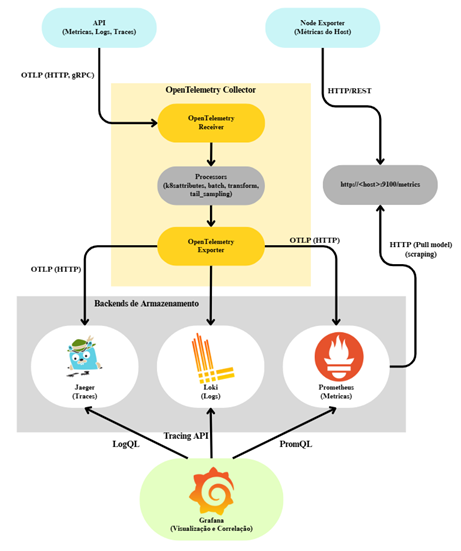
\includegraphics[width=0.65\textwidth]{images/Diagramas/arquitetura_da_solucao.png}
    \caption{Arquitetura da solução de monitorização com OpenTelemetry, Prometheus, Loki, Jaeger e Grafana}
    \label{fig:otel_arch}
\end{figure}

A Figura \ref{fig:otel_arch} ilustra o fluxo de dados de telemetria desde a sua origem nos microsserviços até à visualização final no Grafana. Nesse fluxo, os dados são primeiro gerados e enriquecidos nas aplicações, depois enviados para o \textit{Collector}, onde são processados, transformados e encaminhados para diferentes sistemas de armazenamento, conforme o seu tipo (métricas, logs ou \textit{traces}). Finalmente, o Grafana agrega estes dados e proporciona uma visualização unificada para análise operacional e diagnóstico. Esta divisão clara entre instrumentação, processamento e visualização confere ao sistema maior flexibilidade e evita o acoplamento entre os serviços da aplicação e a infraestrutura de monitorização.

\subsubsection{APIs e SDKs}
As API definem os contratos para a geração e correlação de dados de telemetria. Os SDK são implementações específicas de linguagem das APIs, fornecendo as ferramentas necessárias para instrumentar o código das aplicações. Estes SDK permitem aos utilizadores gerar dados de telemetria na sua linguagem de programação escolhida e exportá-los para um backend preferencial. Incluem bibliotecas de instrumentação que geram dados relevantes a partir de bibliotecas e frameworks populares (por exemplo, requisições HTTP) e detetores de recursos que adicionam atributos contextuais (como nome do pod ou namespace em Kubernetes) aos dados de telemetria (OpenTelemetry Authors, 2025; Thakur \& Chandak, 2022).

\subsubsection{Collector}
O OpenTelemetry Collector é um componente independente e agnóstico de fornecedor, concebido para receber, processar e exportar dados de telemetria. Atua como um hub centralizado para gerir pipelines de telemetria, recebendo dados em vários formatos (como OTLP, Prometheus, Jaeger) e encaminhando-os para um ou mais backends. A sua capacidade de processar e filtrar dados antes da exportação otimiza o fluxo de dados, reduzindo a sobrecarga nas aplicações e melhorando a eficiência geral (OpenTelemetry Authors, 2025; Thakur \& Chandak, 2022).

\subsubsection{Exportadores (Exporters)}
Os exportadores são componentes responsáveis por enviar os dados de telemetria (após serem gerados pelas aplicações ou processados pelo Collector) para ferramentas de backend específicas, como Grafana, Jaeger, Prometheus, Loki ou outros sistemas proprietários. A utilização de exportadores OTLP é considerada uma boa prática, pois são concebidos para emitir dados OpenTelemetry sem perda de informação e são amplamente suportados por diversas plataformas de monitorização (OpenTelemetry Authors, 2025; Thakur \& Chandak, 2022).

\subsubsection{Node Exporter}
O Node Exporter é utilizado como agente de monitorização ao nível do sistema operativo, responsável por expor métricas relacionadas com CPU, memória, disco e rede. Embora não esteja diretamente integrado no pipeline do \textit{OpenTelemetry Collector}, este componente fornece ao Prometheus dados cruciais sobre a infraestrutura subjacente, permitindo complementar a monitorização das aplicações com indicadores do ambiente de execução.

Inicialmente, tentou-se recolher estas métricas através do \textit{OpenTelemetry Collector}, de forma a centralizar todo o processo de monitorização, incluindo as métricas de infraestrutura num único pipeline de recolha e exportação. A intenção era utilizar o Collector como ponto único de integração, encaminhando todos os dados para os respetivos backends (Prometheus, Loki e Jaeger).

Contudo, durante a implementação, verificou-se que a configuração do Collector para recolher métricas do sistema operativo exigia componentes e \textit{receivers} adicionais, cuja compatibilidade e maturidade ainda se encontram limitadas. Para além disso, o nível de detalhe e granularidade obtido não correspondia ao fornecido pelo Node Exporter, tornando essa abordagem menos prática.

Por este motivo, optou-se por manter o Node Exporter como fonte dedicada para métricas de sistema, uma vez que a sua integração direta com o Prometheus é simples, amplamente documentada e de implementação imediata. Assim, o \textit{OpenTelemetry Collector} permanece responsável pela recolha e encaminhamento dos dados das aplicações (métricas, logs e \textit{traces}) para os seus destinos (Prometheus, Loki e Jaeger). Esta abordagem revelou-se mais simples, estável e adequada ao objetivo de obter uma visão completa tanto da infraestrutura como das aplicações.


\subsubsection{Camada de Visualização e Análise}
O Grafana atua como uma interface de utilizador unificada para visualizar e analisar os dados. Esta ferramenta integra os backends (Prometheus, Loki e Jaeger), permitindo a criação de dashboards interativos que mostram as métricas, logs e traces de maneira correlacionada, facilitando o diagnóstico e a tomada de decisões operacionais.


\subsection{Fluxo de Telemetria}

O fluxo de dados de telemetria segue um \textit{pipeline} bem definido que separa instrumentação, recolha, processamento e armazenamento/visualização, conforme ilustrado na Figura \ref{fig:pipeline_otel}. Esta organização permite correlação ponta a ponta com baixo acoplamento aos \textit{backends}.

\begin{enumerate}
    \item A aplicação \textit{ASP.NET Core} emite telemetria (logs, métricas, \textit{traces}) via \textit{OTLP gRPC} e envia-a para o \textit{receiver} do \textit{OpenTelemetry Collector}.
    \item As métricas do sistema operativo são recolhidas diretamente pelo \textit{Prometheus} através do \textit{Node Exporter}.
    \item O \textit{OTel Receiver} aceita entradas de diferentes fontes, incluindo \textit{OTLP} e \textit{scraping} do \textit{Prometheus}.
    \item Os dados são encaminhados para os \textit{processors} do \textit{Collector}, que executam transformação (\textit{transform}), enriquecimento de atributos (\textit{attributes}), agregação (\textit{batch}) e amostragem de \textit{traces} (\textit{tail\_sampling}).
    \item Após o processamento, os dados são enviados pelos \textit{exporters} para os respetivos destinos: \textbf{Logs} $\rightarrow$ \textit{Loki}, \textbf{Traces} $\rightarrow$ \textit{Jaeger} e \textbf{Métricas} $\rightarrow$ \textit{Prometheus}.
    \item O \textit{Grafana} atua como ponto de agregação visual, utilizando as linguagens de consulta específicas de cada \textit{backend} (PromQL, LogQL, \textit{Tracing API}) para gerar \textit{dashboards} interativos e correlações.
\end{enumerate}


\begin{figure}[H]
\centering
\resizebox{\linewidth}{!}{%
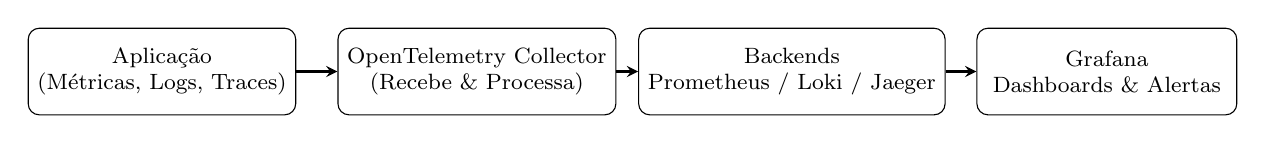
\begin{tikzpicture}[>=stealth,
    box/.style={rectangle,rounded corners,draw,minimum height=1.1cm,minimum width=3.3cm,align=center,font=\footnotesize}]
\node[box] (app) at (0,0) {Aplicação\\(Métricas, Logs, Traces)};
\node[box] (otel) at (4,0) {OpenTelemetry Collector\\(Recebe \& Processa)};
\node[box] (back) at (8,0) {Backends\\Prometheus / Loki / Jaeger};
\node[box] (graf) at (12,0) {Grafana\\Dashboards \& Alertas};
\draw[->,thick] (app)--(otel); \draw[->,thick] (otel)--(back); \draw[->,thick] (back)--(graf);
\end{tikzpicture}%
}
\caption{Pipeline simplificado de telemetria na arquitetura implementada}
\label{fig:pipeline_otel}
\end{figure}


\section{Detalhes Técnicos da Implementação}

\subsection{Estratégia de Instrumentação em .NET}

Do ponto de vista técnico, a instrumentação foi aplicada exclusivamente aos serviços criados internamente, evitando a recolha de dados de dependências externas. Desta forma, métricas, logs e traces refletem apenas o comportamento dos microsserviços proprietários, reduzindo o ruído e a sobrecarga de dados. Esta abordagem garante que a telemetria recolhida é relevante para a análise e otimização da plataforma R2UT, focando a monitorização nos elementos críticos sob responsabilidade direta da equipa de desenvolvimento.

A instrumentação de aplicações é um passo crucial para gerar dados de telemetria significativos. Em ambientes de microsserviços com múltiplas APIs, a instrumentação individual de cada serviço pode ser repetitiva e propensa a erros. Para mitigar esta complexidade, foi adotada uma abordagem prática e reutilizável para a instrumentação de APIs ASP.NET Core, utilizando um pacote comum (\textit{DTX.Base.Common}). Este pacote encapsula toda a configuração necessária para a emissão de \textit{traces} distribuídos, métricas e logs estruturados, promovendo uma padronização e um desacoplamento eficaz entre o código da aplicação e a infraestrutura de monitorização.

Esta estratégia centraliza a lógica de monitorização num único ponto, reduzindo significativamente o código repetido. A configuração da telemetria pode ser ativada e controlada dinamicamente através de variáveis de ambiente, conferindo flexibilidade e portabilidade entre diferentes ambientes (desenvolvimento, homologação e produção). Para instrumentar novos serviços, a intervenção necessária é mínima: basta adicionar o pacote \textit{DTX.Base.Common}, invocar um método de extensão no \texttt{Program.cs} e definir as variáveis de ambiente correspondentes.

A lógica de monitorização foi centralizada num único método de extensão, aplicado na inicialização de cada API \.NET:

\begin{verbatim}
builder.ConfigureOpenTelemetry();
\end{verbatim}

Este método ativa automaticamente os componentes do OpenTelemetry responsáveis pela instrumentação de \textit{tracing} distribuído, recolha de métricas e exportação de logs estruturados. As opções de configuração são controladas dinamicamente por variáveis de ambiente, evitando alterações no código ou recompilação ao migrar entre ambientes.


As variáveis de ambiente listadas na Tabela \ref{tab:otel_env_vars} são responsáveis por configurar a camada de exportação OTLP em cada microsserviço. Em vez de definir endpoints ou credenciais diretamente no código, estes parâmetros são injetados no ambiente de execução, permitindo separar configuração operacional da lógica de aplicação.

A variável \texttt{OTEL\_EXPORTER\_OTLP\_ENDPOINT} determina o endereço do Collector para onde os dados serão enviados, garantindo flexibilidade na migração entre ambientes (por exemplo, ambiente local, cluster de homologação ou produção em Kubernetes). A variável \texttt{OTEL\_EXPORTER\_OTLP\_PROTOCOL} define o protocolo de comunicação a utilizar, assegurando compatibilidade com diferentes configurações de rede e segurança. Por fim, \texttt{OTEL\_EXPORTER\_OTLP\_HEADERS} permite incluir cabeçalhos adicionais, como tokens de autenticação ou etiquetas de contexto, possibilitando uma integração segura e multi-tenant quando necessário.

Este modelo de configuração facilita a automação de \textit{deploys}, promove maior segurança operacional e reduz a necessidade de alterações no código ao longo do ciclo de vida do sistema.


\begin{table}[H]
\centering
\begin{tabular}{|p{6cm}|p{8cm}|}
\hline
\textbf{Variável} & \textbf{Descrição} \\ \hline
\texttt{OTEL\_EXPORTER\_OTLP\_ENDPOINT} & URL do \textit{endpoint} do Collector OTLP. \\ \hline
\texttt{OTEL\_EXPORTER\_OTLP\_PROTOCOL} & Protocolo utilizado (\textit{grpc} ou \textit{http/protobuf}). \\ \hline
\texttt{OTEL\_EXPORTER\_OTLP\_HEADERS} & Cabeçalhos opcionais no formato chave=valor (ex.: \texttt{Authorization=Bearer abc}). \\ \hline
\end{tabular}
\caption{Variáveis de ambiente utilizadas para configuração da exportação OTLP}
\label{tab:otel_env_vars}
\end{table}

Embora a instrumentação explícita via \texttt{DTX.Base.Common} fosse o padrão adotado, também foi avaliada a possibilidade de implementação da instrumentação \textit{zero-code} no ambiente .NET, utilizando agentes e configurações automáticas do \textit{OpenTelemetry}. No entanto, foram identificadas algumas limitações no controlo da granularidade dos dados e na integração com determinadas bibliotecas utilizadas internamente. Por esse motivo, optou-se por encapsular a instrumentação num pacote comum, garantindo padronização e flexibilidade.


\subsection{Vantagens da Abstração da Instrumentação OpenTelemetry}

O encapsulamento da lógica de instrumentação no pacote \texttt{DTX.Base.Common} e a exposição via um método de extensão (\texttt{ConfigureOpenTelemetry()}) proporcionam benefícios significativos para o desenvolvimento e a operação de aplicações distribuídas. De referir:

\begin{itemize}
\item \textbf{Padronização da Instrumentação entre Múltiplas APIs}, que garante que todas as APIs sigam as mesmas convenções de observabilidade, resultando em dados de telemetria consistentes e facilmente comparáveis. Isso é fundamental para a correlação eficaz de dados em sistemas complexos.

\item \textbf{Desacoplamento da Infraestrutura de Monitorização}, que faz com que o código da aplicação se torne independente das ferramentas de backend utilizadas (\textit{Grafana}, \textit{Jaeger}, \textit{Tempo}, etc.). Se houver uma mudança nas ferramentas de monitorização, as modificações são minimizadas e confinadas à configuração do Collector ou às variáveis de ambiente, não exigindo alterações no código da aplicação.

\item \textbf{Facilidade de Configuração via Ambiente}, que assegura que a ativação e o ajuste da observabilidade sejam feitos através de variáveis de ambiente, o que simplifica a implantação e a gestão em diferentes ambientes (desenvolvimento, homologação, produção), promovendo a portabilidade.

\item \textbf{Redução Significativa de Código Repetido}, que, ao centralizar a lógica de observabilidade num único ponto, evita a duplicação de código em cada novo serviço ou API, tornando o processo de instrumentação mais eficiente e menos propenso a erros.
\end{itemize}

Com esta abordagem, a instrumentação de novos serviços pode ser realizada com mínima intervenção, com a adição do pacote \texttt{DTX.Base.Common}, uma chamada simples ao método de extensão no \texttt{Program.cs} e a definição das variáveis de ambiente necessárias. Isso acelera o desenvolvimento e garante que a monitorização seja uma parte integrante do ciclo de vida da aplicação desde o início.

\break

\section{Coleta de dados com o OpenTelemetry Collector}

A fase de coleta é o ponto de entrada para os dados de telemetria no pipeline de monitorização. É responsável por capturar logs, métricas e traces gerados pelas aplicações instrumentadas, agentes \textit{sidecar} ou ferramentas de terceiros. A coleta é feita principalmente através dos \textit{receivers} do \textit{OpenTelemetry Collector}, que atuam como ouvintes ou \textit{scrapers}, aceitando dados em vários formatos.

O \textit{OpenTelemetry Collector}, um componente central do ecossistema, funciona como um hub de processamento centralizado, capaz de lidar com múltiplas fontes e destinos de dados. Na implementação em questão, o Collector foi configurado para escutar em duas portas principais para o protocolo OTLP: \texttt{4317} para \texttt{gRPC} e \texttt{4318} para \texttt{HTTP}. Esta configuração permite que as aplicações enviem telemetria usando o protocolo de sua preferência. A fase de coleta é crítica, uma vez que é ela que garante que os dados cheguem de forma consistente e em tempo real ao pipeline de monitorização.

No ambiente \textit{Kubernetes}, a implantação do \textit{OpenTelemetry Collector} foi realizada como um \textit{DaemonSet}. Esta escolha de implantação garante que o Collector seja executado como um agente em cada nó (\textit{node}) do cluster, em vez de ser um serviço centralizado. Cada instância do \textit{DaemonSet Collector}, que age como um agente local, recebe a telemetria dos pods que estão no mesmo nó.

A principal vantagem desta abordagem é a redução de latência e a garantia de segurança. Ao coletar a telemetria localmente, os dados não precisam viajar pela rede do cluster, reduzindo a latência e o risco de congestionamento. Além disso, essa arquitetura de agente local é mais resiliente, pois a falha de um agente afeta apenas a coleta de dados de um único nó, enquanto os outros nós continuam a operar normalmente. Essa configuração de \textit{DaemonSet}, combinada com os \textit{receivers} do Collector, otimiza o fluxo de telemetria e torna-o mais robusto e eficiente.

\subsection{O Protocolo OTLP (gRPC/HTTP)}

O \textit{OpenTelemetry Protocol} (OTLP) é o protocolo padrão utilizado na plataforma de observabilidade para o transporte de dados de telemetria, como métricas, logs e \textit{tracing} distribuído. Desenvolvido como parte do ecossistema OpenTelemetry, o OTLP é um protocolo aberto, extensível e eficiente, que permite a comunicação entre aplicações instrumentadas, agentes de coleta como o \textit{OpenTelemetry Collector}, e sistemas de backend, como o \textit{Grafana Loki} (logs), o \textit{Jaeger} (traces) ou \textit{Prometheus} (métricas). O protocolo suporta os formatos \texttt{gRPC} e \texttt{HTTP/protobuf}, garantindo flexibilidade de integração com diversos ambientes e ferramentas. Num cluster Kubernetes, o uso do OTLP padroniza a coleta e exportação de dados de observabilidade entre os pods e os componentes da infraestrutura de monitorização, garantindo portabilidade, interoperabilidade e escalabilidade da solução implementada.

\subsection{OpenTelemetry Operator}

Gerir a observabilidade em ambientes Kubernetes pode tornar-se complexo, especialmente quando é necessário configurar múltiplos Collectors, manter consistência de \textit{pipelines} e aplicar boas práticas de escalabilidade e de segurança. Para simplificar esta gestão, a comunidade desenvolveu o \textit{OpenTelemetry Operator}, um \textit{Custom Kubernetes Operator} que automatiza o ciclo de vida dos Collectors e a sua configuração.

O \textit{OpenTelemetry Operator} expande o Kubernetes através de \textit{Custom Resource Definitions} (CRDs), introduzindo novos tipos de recurso que descrevem configurações de observabilidade de forma declarativa. O recurso mais importante é o \texttt{OpenTelemetryCollector}, no qual o utilizador define, em YAML, as características desejadas do Collector (\textit{receivers}, \textit{processors}, \textit{exporters} e modo de execução). O Operator traduz automaticamente essa especificação em objetos nativos do Kubernetes, como \textit{Deployments}, \textit{DaemonSets} ou \textit{ConfigMaps}. Dessa forma:

\begin{enumerate}
\item O programador ou DevOps aplica um manifesto \texttt{OpenTelemetryCollector};
\item O Operator valida e cria os recursos Kubernetes correspondentes;
\item O Collector é implantado de forma consistente e conforme as boas práticas definidas pela comunidade.
\end{enumerate}


O recurso \texttt{OpenTelemetryCollector}, disponibilizado pelo \textit{OpenTelemetry Operator}, permite definir, de forma declarativa, o modo de execução do Collector, conferindo elevada flexibilidade na adaptação da arquitetura de monitorização às características do sistema. Os principais modos de operação são:

\begin{itemize}
    \item \textbf{DaemonSet.} Executa uma instância do Collector em cada nó do cluster, recolhendo a telemetria localmente e reduzindo a latência e o tráfego de rede. Este modo é particularmente indicado para clusters de grande dimensão ou aplicações com elevado volume de métricas e logs.

    \item \textbf{Deployment.} Executa o Collector como um serviço centralizado, atuando como \textit{gateway} e agregando telemetria antes de a reenviar para os backends definidos. É uma opção recomendada para ambientes de desenvolvimento ou para arquiteturas onde a centralização seja operacionalmente vantajosa.

    \item \textbf{Sidecar.} Executa o Collector em conjunto com cada \textit{pod}, garantindo o nível máximo de isolamento e controlo sobre a instrumentação de cada serviço. Este modelo oferece monitorização altamente granular, embora com maior custo de recursos.

    \item \textbf{StatefulSet.} Utilizado em cenários onde é necessário garantir estado persistente ou uma configuração estável e ordenada, útil em pipelines de telemetria mais complexos ou ambientes de auditoria.
\end{itemize}

Além desta flexibilidade arquitetural, a utilização do \textit{OpenTelemetry Operator} oferece benefícios adicionais:


\begin{itemize}
    \item \textbf{Automação.} Elimina a necessidade de escrever e manter manualmente manifestos Kubernetes complexos para cada instância do Collector, simplificando significativamente a gestão operacional e reduzindo o risco de erros de configuração.

    \item \textbf{Consistência e padronização.} Garante que todas as instâncias do Collector são configuradas de forma homogénea e alinhadas com boas práticas, assegurando uniformidade na recolha e processamento da telemetria em todo o cluster.

    \item \textbf{Integração nativa com GitOps.} Por ser baseado em definições declarativas, integra-se facilmente com pipelines de CI/CD e ferramentas GitOps, como ArgoCD e Flux, facilitando a gestão versionada e auditável das configurações de monitorização.

    \item \textbf{Evolução contínua e alinhamento com a comunidade.} O Operator é mantido pela comunidade OpenTelemetry, garantindo compatibilidade com novas versões, boas práticas atualizadas e reduzindo o risco de configurações obsoletas ao longo do tempo.
\end{itemize}


Em síntese, o \textit{OpenTelemetry Operator} simplifica substancialmente a adoção de monitorização em Kubernetes, promovendo maior automação, padronização e escalabilidade, ao mesmo tempo que reduz o esforço manual e a probabilidade de erros operacionais.

\begin{figure}[H]
    \centering
    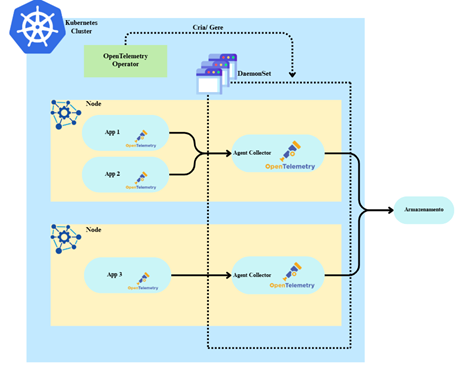
\includegraphics[width=0.8\textwidth]{images/Diagramas/daemonset_collector.png}
    \caption{Arquitetura de coleta local com \textit{OpenTelemetry Collector} em modo \textit{DaemonSet}.}
    \label{fig:otel-daemonset}
\end{figure}


A abordagem adotada neste trabalho foi a execução do \textit{OpenTelemetry Collector} como um \textit{DaemonSet}, disponibilizando um agente local em cada nó do cluster Kubernetes (Figura \ref{fig:otel-daemonset}). Em cada nó, um \textit{Pod} do Collector expõe \textit{receivers} OTLP por gRPC (porta 4317) e HTTP/Protobuf (porta 4318), recebendo métricas, logs e traces das \textit{workloads} residentes nesse nó.

Esta decisão foi guiada por três objetivos principais:

\begin{itemize}
    \item \textbf{Baixa latência na entrega de telemetria} --- evitando transmissões de rede adicionais antes do primeiro processamento;
    \item \textbf{Resiliência local} --- confinando o impacto de eventuais falhas ao nó específico, sem afetar o resto do cluster;
    \item \textbf{Simplicidade de integração} --- permitindo que as aplicações publiquem telemetria para um único \textit{endpoint} local, sem a necessidade de mecanismos adicionais de descoberta.
\end{itemize}

A adoção do padrão \textit{DaemonSet} resultou numa menor variabilidade na entrega dos sinais, com coleta e pré-processamento a nível local, isolamento de falhas por nó, redução da dependência de rede intra-cluster e uma configuração simplificada do lado das aplicações, uma vez que estas comunicam com um \textit{endpoint} local único.


\section{Processamento e Transformação dos Dados}

Após a sua recolha, os dados de telemetria passam por uma fase crítica de processamento dentro do \textit{OpenTelemetry Collector}. Esta etapa, orquestrada por diversos \textit{processors}, é essencial para modificar, enriquecer, agrupar ou filtrar os dados, assegurando a sua consistência, eficiência e utilidade para os sistemas subsequentes de armazenamento e análise.


\subsection{Processadores e as suas Aplicações}

Após a fase de recolha, os dados de telemetria passam por um estágio fundamental de processamento dentro do \textit{OpenTelemetry Collector}. Este processamento é realizado por um conjunto de \textit{processors}, responsáveis por transformar, enriquecer, agrupar e filtrar os dados. Esta etapa assegura que a telemetria seja consistente, eficiente e alinhada com as necessidades de análise, conformidade e desempenho da solução implementada.

De forma a consolidar o papel de cada componente, a Tabela \ref{tab:otel-processors} apresenta os principais \textit{processors} utilizados, a sua função primária e respetivas aplicações práticas.

\begin{table}[H]
\centering
\caption{Principais \textit{processors} do OpenTelemetry Collector utilizados}
\label{tab:otel-processors}
\begin{tabular}{|p{3cm}|p{4cm}|p{4.2cm}|p{4.2cm}|}
\hline
\textbf{Processor} & \textbf{Função Primária} & \textbf{Aplicações Chave} & \textbf{Benefício para Monitorização} \\ \hline
\texttt{transform} & Modifica dados com OTTL. & Adiciona \texttt{service.name}, normaliza severidade, converte timestamps. & Consistência semântica e refinamento da telemetria. \\ \hline
\texttt{batch} & Agrupa dados em lotes. & Reduz chamadas de rede e overhead. & Melhora o débito e otimiza a exportação. \\ \hline
\texttt{attributes} & Adiciona ou altera atributos. & Injeta metadados como ambiente e host. & Melhora correlação, filtragem e contexto. \\ \hline
\texttt{resource} & Modifica atributos de recurso. & Garante aplicação uniforme de \texttt{service.name}, versão, ambiente. & Uniformidade e correta identificação de origem dos dados. \\ \hline
\texttt{memory\_limiter} & Controla consumo de memória. & Evita saturação e falha do Collector. & Estabilidade operacional. \\ \hline
\texttt{tail\_sampling} & Amostragem com base no trace completo. & Seleciona traces críticos (ex.: erros, alta latência). & Reduz volume e custo mantendo visibilidade de incidentes. \\ \hline
\end{tabular}
\end{table}

\begin{itemize}
% [label=\textbf{\arabic*.}, leftmargin=1.2cm]

\item \textbf{Processador \texttt{transform}}\\
% \subsubsection{Processador \texttt{transform}}

O processador \texttt{transform} utiliza a \textit{OpenTelemetry Transformation Language} (OTTL) para realizar modificações avançadas nos dados de telemetria. Na implementação atual, é utilizado para adicionar o atributo \texttt{service.name} aos sinais de telemetria, converter \textit{timestamps} para um formato padronizado, normalizar níveis de severidade de logs (por exemplo, mapeando diferentes níveis para categorias consistentes como \texttt{INFO}, \texttt{WARN} e \texttt{ERROR}), e aplicar regras de amostragem dinâmica a \textit{traces}. No entanto, devido ao seu elevado grau de flexibilidade e poder expressivo, a sua configuração deve ser cuidadosamente validada para evitar \textit{transformações inconsistentes} (\textit{Unsound Transformations}) ou \textit{conflitos de identidade} (\textit{Identity Conflicts}), que podem comprometer a integridade e a fiabilidade da telemetria.

\clearpage

\item \textbf{Processador \texttt{batch}}\\
% \subsubsection{Processador \texttt{batch}}

Este processador agrupa eficientemente os dados de telemetria em lotes antes de serem exportados. O batching reduz significativamente o número de chamadas de rede e a sobrecarga associada, melhorando assim o débito geral e a eficiência da exportação de dados, especialmente em ambientes de alto volume

\item \textbf{Processador \texttt{attributes}}\\
% \subsubsection{Processador \texttt{attributes}}

O processador \texttt{attributes} permite adicionar, modificar ou remover atributos (metadados) associados a \textit{spans}, logs ou métricas. Na prática, este processador é utilizado para enriquecer os dados de telemetria com informação contextual relevante - por exemplo, injetando um atributo estático que identifica o ambiente de execução (como \textit{produção} ou \textit{desenvolvimento}) ou acrescentando metadados ao nível do \textit{host}. Este enriquecimento é fundamental para consultas mais eficientes, filtragem precisa e correlação robusta entre diferentes sinais, contribuindo para uma análise mais clara e completa do comportamento do sistema distribuído.

\item \textbf{Processador \texttt{resource}}\\
% \subsubsection{Processador \texttt{resource}}


Este processador tem como objetivo a modificação de atributos de recurso, os quais descrevem a entidade responsável pela geração da telemetria, como o serviço da aplicação, a máquina \textit{host} ou o \textit{container}. É essencial para anexar de forma consistente metadados fundamentais, tais como \textit{environment}, \textit{service version} ou \textit{region} às métricas e para enriquecer logs com informação contextual detalhada. O processador \texttt{resource} assegura que atributos de identificação comuns, nomeadamente \texttt{service.name}, são aplicados uniformemente a todos os sinais de telemetria (logs, \textit{traces} e métricas). Esta consistência é crucial para permitir uma correlação eficiente e precisa entre sinais no Grafana.

\item \textbf{Processador \texttt{memory\_limiter}}\\
% \subsubsection{Processador \texttt{memory\_limiter}}

Este processador é utilizado para evitar que o OpenTelemetry Collector consuma uma quantidade excessiva de memória. Ao definir limites explícitos de utilização, previne que o processo do Collector falhe devido ao esgotamento de recursos, garantindo assim a estabilidade e a fiabilidade contínuas de todo o \textit{pipeline} de monitorização. Esta salvaguarda é especialmente importante em ambientes de elevada carga, onde picos de telemetria podem ocorrer de forma imprevisível.


\item \textbf{Processador \texttt{tail\_sampling}}\\
% \paragraph{Processador \texttt{tail\_sampling}.}

Este processador permite tomar decisões de amostragem com base no contexto completo de um \textit{trace}, ou seja, apenas após todos os \textit{spans} associados terem sido recebidos. Suporta múltiplos critérios de filtragem que podem ser combinados, incluindo amostragem baseada na latência observada, taxas probabilísticas, códigos de estado HTTP (por exemplo, apenas \textit{traces} com erro) ou limites de taxa. 

Esta abordagem de amostragem baseada no contexto completo do trace é fundamental para controlar o volume de dados gerados por sistemas distribuídos de elevado tráfego, permitindo reter apenas os \textit{traces} mais relevantes para diagnóstico e análise. O seu uso contribui para otimizar custos de armazenamento e melhorar o desempenho de consultas no \textit{backend} de \textit{tracing}, mantendo a capacidade de capturar e investigar \textit{traces} críticos ou anómalos.

\end{itemize}

A capacidade do \textit{OpenTelemetry Collector} de modificar todos os aspetos da telemetria, incluindo a remoção de informações sensíveis através do processador \texttt{transform} ou o enriquecimento consistente de dados com atributos específicos, posiciona-o como um ponto de controlo estratégico na governação de dados. Esta centralização do controlo significa que os requisitos de conformidade podem ser geridos e aplicados ao nível do Collector, reduzindo a necessidade de alterações individuais nas aplicações ou de configurações complexas específicas dos \textit{backends}.

Esta abordagem não só centraliza significativamente o controlo de dados, como também minimiza a superfície de ataque para fugas acidentais de informação. Além disso, a capacidade de filtrar, agrupar e reduzir a cardinalidade dos dados antes da sua exportação para os \textit{backends} traduz-se diretamente em poupanças substanciais nos custos de ingestão e armazenamento, especialmente em serviços de observabilidade geridos. Ao reduzir o volume e a complexidade dos dados na origem, o Collector melhora o desempenho das consultas nos \textit{backends} e mitiga potenciais problemas de ``crise de identidade'' em métricas, resultando em \textit{dashboards} mais fiáveis. Assim, o Collector assume-se como um componente crítico para assegurar tanto a eficiência económica como a eficiência operacional de toda a \textit{stack} de monitorização.



\section{Persistência e Armazenamento de Dados }

A seleção dos sistemas de \textit{backend} para armazenar \textit{logs}, \textit{traces} e métricas foi realizada de acordo com os requisitos definidos pela empresa, que recomendou soluções maduras e amplamente adotadas no ecossistema de monitorização. Estas ferramentas foram utilizadas exclusivamente como \textit{backends}, tendo como principal objetivo centralizar o armazenamento e a análise dos dados exportados pelos microsserviços, sem adicionar dependências diretas ao código das aplicações.

\subsection{Armazenamento de \textit{Logs} com o Loki}
O Loki foi escolhido como sistema de armazenamento de \textit{logs} devido à sua arquitetura otimizada para consultas baseadas em etiquetas (\textit{labels}), em vez de pesquisa textual completa (\textit{full-text search}). Esta abordagem torna-o mais eficiente e menos dispendioso em termos de recursos quando comparado com soluções tradicionais, como o Elasticsearch. 

Os \textit{logs} estruturados emitidos pelas APIs .NET são enviados ao \textit{OpenTelemetry Collector} através do protocolo OTLP e, posteriormente, exportados para o Loki. A integração nativa com o Grafana permite que os \textit{logs} sejam visualizados e correlacionados com métricas e \textit{traces}, proporcionando uma análise centralizada e coerente do sistema.

\subsection{Armazenamento de \textit{Traces} com o Jaeger}
O Jaeger foi adotado como \textit{backend} de armazenamento e análise de \textit{traces} distribuídos, dada a sua capacidade comprovada de fornecer visibilidade \textit{end-to-end} sobre o ciclo de vida de uma requisição. Com base no atributo \texttt{service.name}, é possível segmentar e filtrar os \textit{traces}, identificando gargalos e potenciais pontos de falha durante a interação entre microsserviços.

Os dados são exportados pelo \textit{OpenTelemetry Collector} via OTLP/\textit{gRPC} para o \textit{endpoint} do Jaeger, onde ficam persistidos para consulta e inspeção detalhada, sendo posteriormente visualizados através do Grafana.

\subsection{Armazenamento de Métricas com o Prometheus}
O Prometheus foi selecionado como sistema de armazenamento de métricas devido à sua robustez no processamento de séries temporais e à linguagem de consulta PromQL, que possibilita análises avançadas e precisas. As métricas das aplicações .NET são recolhidas pelo \textit{OpenTelemetry Collector} e exportadas para o Prometheus, evitando exposição direta dos serviços e centralizando a captura de telemetria.

Complementarmente, as métricas de infraestrutura provenientes do \textit{Node Exporter} são recolhidas diretamente pelo Prometheus através de \textit{scraping} HTTP. Esta abordagem combinada assegura visibilidade tanto ao nível da aplicação como da infraestrutura, proporcionando uma visão abrangente e consistente do desempenho do sistema.
